\chapter*{Addendum: sRNA-induced synthetic translational bursting in bacteria}
\phantomsection
\addcontentsline{toc}{chapter}{\protect\numberline{}Addendum: sRNA-induced synthetic translational bursting in bacteria}

\begin{flushright}
    \textit{All the effects of Nature are only the mathematical\\consequences of a small number of immutable laws.}\\
    --- Pierre-Simon Laplace
\end{flushright}

\vspace{1cm}

\noindent This addendum complements the central theme of the thesis, which delves deeply into the macroscopic evolutionary processes in viruses and their stochastic underpinnings, by shifting the focus to the microscopic origins of biological noise. The stochastic nature of evolution is driven by complex interactions among population dynamics, molecular mechanisms, and environmental fluctuations. Within this broader framework, gene expression represents a fundamental, intrinsically noisy process whose randomness propagates upward to influence larger-scale phenomena such as evolution. Here, the addendum examines a specific molecular mechanism: translational bursting in gene expression, using synthetic sRNA systems in \textit{E. coli} as a model. The examination of the mechanisms by which these systems induce and regulate cellular bursts offers a glimpse into the complex molecular mechanisms underlying biological noise and provides valuable insights into how molecular stochasticity propagates into evolutionary dynamics. This supports the contention that a multiscale perspective on randomness is essential for understanding and harnessing the intricacies of biological function.\\

\noindent To date, this work has not been published in a peer-reviewed journal.\\

\vfill

% \noindent\textbf{Goiriz L},  Montagud-Martínez R, Dolcemascolo R, Ruiz R, Rodrigo G. \textit{In preparation}.\\

\pagebreak

\noindent Further reading on related works to which I contributed, and whose methodologies are based on similar principles, can be found in the following references:\\

\noindent Dolcemascolo R, \textbf{Goiriz L}, Montagud-Martínez R, Rodrigo G. (2022) \href{https://doi.org/10.1371/journal.pcbi.1010087}{Gene regulation by a protein translation factor at the single-cell level}. \textit{PLoS Comput. Biol.}, 18(5): e1010087.\\

\noindent Dolcemascolo R, Heras-Hernández M, \textbf{Goiriz L}, Montagud-Martínez R, Requena-Menéndez A, Ruiz R, Pérez-Ràfols A, Higuera-Rodríguez R.A, Pérez-Ropero G, Vranken W.F, Martelli T, Kaiser W, Buijs J, Rodrigo G. (2024) \href{https://doi.org/10.7554/eLife.91777.3}{Repurposing the mammalian RNA-binding protein Musashi-1 as an allosteric translation repressor in bacteria}. \textit{eLife}, 12: RP91777.\\

\noindent Dolcemascolo R, Ruiz R, Baldanta S, \textbf{Goiriz L}, Heras-Hernández M, Montagud-Martínez R, Rodrigo G. (2024) \href{https://doi.org/10.1186/s13036-024-00448-x}{Probing the orthogonality and robustness of the mammalian RNA-binding protein Musashi-1 in Escherichia coli}. \textit{J. Biol. Eng.} 18(52).\\

\vfill

\pagebreak

\sloppy

\section*{Introduction}

Gene expression is inherently stochastic, resulting in considerable cell-to-cell variability even among clonal bacterial populations \cite{Elowitz2002,Swain2002}. One major source of this variability is bursting, where transcription or translation occurs in episodic bouts rather than continuously. Single-cell studies in \textit{E. coli} have shown that mRNA synthesis happens in random pulses \cite{Golding2005}, and that protein production occurs in sporadic bursts \cite{Yu2006}. These findings validate theoretical predictions that rare events, such as a promoter switching to an active state, can drive phenotypic heterogeneity, a behavior long described by stochastic models like the random telegraph model \cite{McAdams1997}. Moreover, the intrinsic noise from low copy-number molecules leads to mRNA and protein distributions that deviate from simple Poisson statistics \cite{Paulsson2004}, which is crucial for both understanding genetic circuits and designing robust biotechnological applications \cite{Taniguchi2010}.

While transcriptional bursting, driven by promoter activation kinetics, is well established, recent studies have focused on post-transcriptional bursting (fluctuations arising after mRNA is synthesized). In bacteria, small regulatory RNAs (sRNAs), which are approximately 50-200 nucleotides long, modulate target mRNA translation and stability \cite{Gottesman2004,Waters2009}. In \textit{E. coli}, many sRNAs bind near the 5' untranslated region of mRNAs, often with the assistance of the Hfq chaperone, to block ribosome binding and promote degradation. Unlike protein transcription factors, sRNAs act stoichiometrically, leading to an all-or-none effect on individual mRNAs: a transcript is either sequestered in an inactive sRNA-bound complex (translation ``OFF'') or remains free for translation (translation ``ON''). This binary regulation can result in bursts of protein production when sRNA levels drop or become saturated \cite{Levine2007}.

Mathematical modeling has been key to understanding post-transcriptional bursting. Approaches such as stochastic differential equations and chemical master equation formulations have been employed to capture the dynamics of sRNA-mRNA interactions. Models analogous to the promoter telegraph model describe two states, ``ON'' (mRNA free of sRNA) and ``OFF'' (mRNA bound by sRNA), and can replicate the bursty behavior observed in experiments. The stochastic simulation algorithm, along with analytical methods like linear noise approximation, has clarified how parameters such as binding affinities, transcription and degradation rates determine burst size and frequency. Empirical studies, including single-cell fluorescence and smFISH, have compared these model predictions with experimental data, validating the role of sRNA regulation in modulating gene expression noise \cite{Golding2005,Taniguchi2010,Levine2007,Rodrigo2018}.

Synthetic biology further leverages these insights to both test and harness post-transcriptional regulation. For instance, CRISPR interference (CRISPRi) employs a catalytically inactive Cas9 and guide RNA to reversibly modulate gene activity, mimicking natural on/off switching \cite{Qi2013}. Similarly, synthetic sRNA systems, designed with tailored antisense regions, reproduce natural sRNA mechanisms to control translation \cite{Sharma2012}. Additionally, toehold switch RNAs, engineered mRNA structures that block translation until triggered by a specific RNA, demonstrate how RNA-only systems can be used to construct controllable gene circuits \cite{Green2014,Qian2011}. These synthetic tools provide powerful platforms to investigate the fundamental principles of biological noise from molecular scale up to its propagation to the evolutionary scale.

Here, we harness a set of mutants of the RAJ11 construct, which is is a synthetic riboregulatory system designed to control gene expression at the post-transcriptional level by exploiting base-pairing interactions between a small regulatory RNA (sRNA) and the 5' untranslated region (5' UTR) of a target mRNA \cite{Rodrigo2015}, to empirically assess the phenomenon of post-transcriptional bursting. In this design, the ribosome-binding site on the mRNA is initially sequestered by an intramolecular hairpin, preventing efficient translation. When the sRNA binds to a complementary ``toehold'' region within that hairpin, it causes a conformational rearrangement that liberates the ribosome-binding site and activates translation. We examined multiple variants of this system, including the wild-type RAJ11 design and several engineered mutants with altered sRNA-mRNA binding affinities, to systematically probe how the strength and dynamics of sRNA-mediated repression influence translational bursting. All constructs share the same overall architecture, allowing direct comparisons. Overall, this system serves as a minimal and predictable framework for studying how RNA--RNA interactions, influenced by thermodynamic parameters and sequence accessibility, modulate protein output.



\section*{Results}
%\subsection*{Bursting Dynamics and Mean Expression}
%Our analysis confirms that small RNA (sRNA)-mediated regulation can induce pronounced translational bursting. In the deterministic mean-field limit, the steady-state mRNA level derived from the stochastic model is $\langle x \rangle = c k_m/\gamma_m$ (for gene copy number $c$, transcription rate $k_m$, mRNA decay rate $\gamma_m$). This result assumes the noise term averages to zero and decouples from the mean dynamics. The sRNA introduces an on/off switching in translation: an mRNA is largely translationally off (ribosome-binding site sequestered) until an sRNA binding event toggles it on. Numerically, bursts of protein production occur with frequency $k_{\text{on}}\langle s\rangle$ (proportional to sRNA abundance $\langle s \rangle$) and have a characteristic size of $k_p/k_{\text{off}}$ proteins (with $k_p$ the translation rate and $k_{\text{off}}$ the inactivation rate).

%Stochastic simulations and analysis reveal that while the mean protein levels can remain similar across different sRNA scenarios (due to compensation between burst frequency and size), the noise and distribution shape are highly sensitive to burst dynamics. For the wild-type RAJ11 system (strong sRNA--mRNA binding), the protein distribution was right-skewed and well-fit by a gamma distribution (shape parameter $k\approx3.86$, scale $\theta\approx415$) with high R$^2$ goodness-of-fit (0.963) for the fluorescence histogram. This indicates significant cell-to-cell variability, yet less extreme than an exponential distribution (which would correspond to $k=1$).

\subsection*{Deconvolution of Expression Distributions}
To accurately quantify the protein output distribution, we deconvolved cellular autofluorescence from the total fluorescence measurements to isolate the true protein expression signals from background noise. Single-cell fluorescence measurements of our synthetic sRNA constructs yield unimodal but highly skewed intensity distributions of protein per cell (\textbf{Fig. \ref{fig:figadd.1}}) due to the burst-like nature of protein expression. Without removing the background contribution, these heavy-tailed distributions would be convolved with extrinsic noise from cellular autofluorescence, potentially obscuring their true shape and overestimating cell-to-cell variability that is not due to actual gene expression bursts. By mathematically deconvolving the measured fluorescence data using a control autofluorescence profile, we eliminate this artifact and recover the genuine distribution of protein expression levels. This procedure ensures that analyses of translational bursting (e.g., determining burst sizes and frequencies) reflect actual biological variability rather than measurement noise, thereby allowing accurate quantification of the noise characteristics inherent to the sRNA-regulated system.


\begin{figure}[ht!]
    \centering
    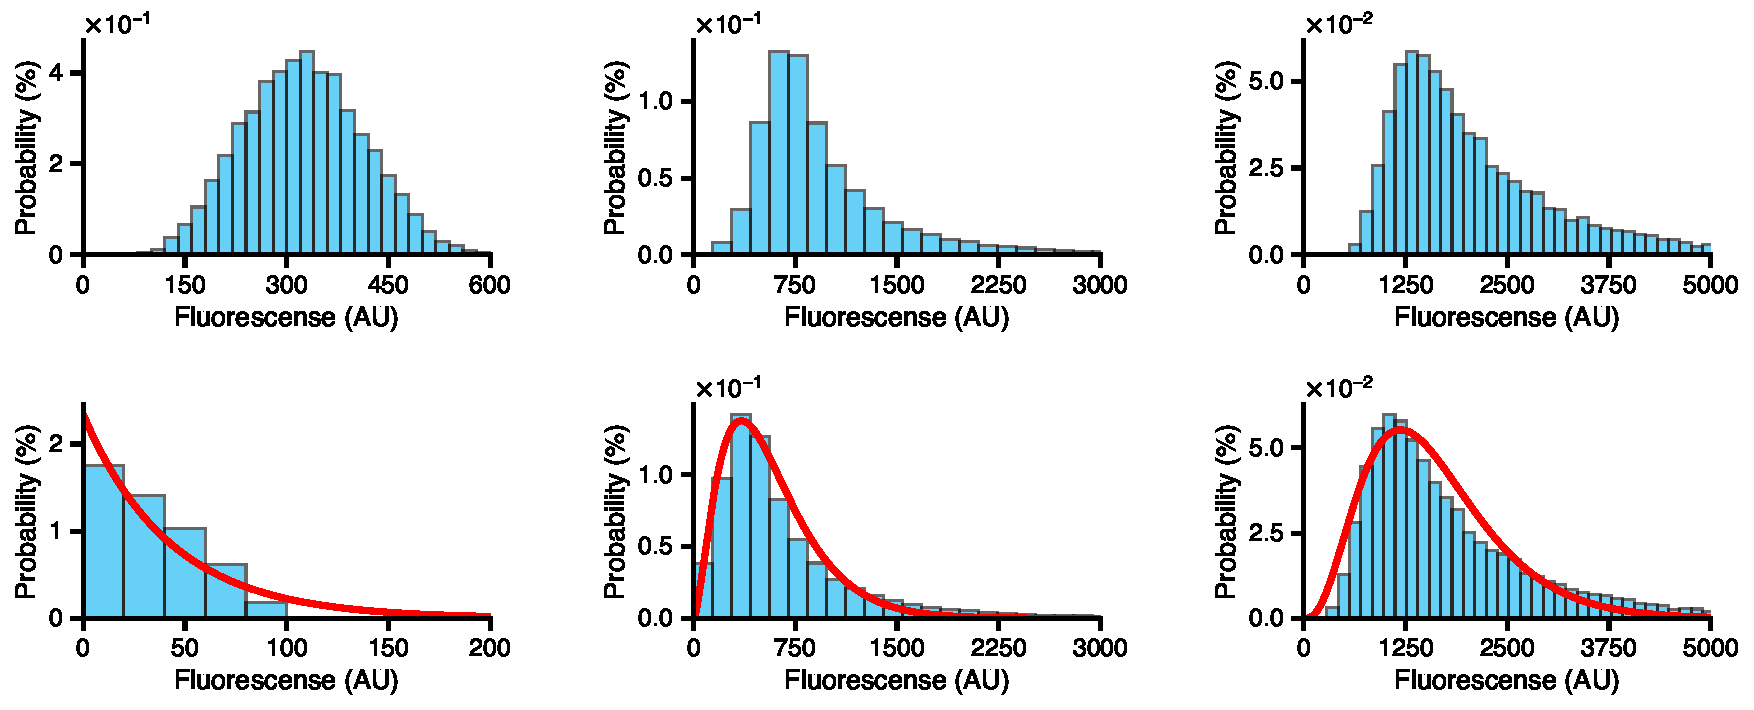
\includegraphics[width=\linewidth]{assets/addendumFig1.pdf}
    \caption{Histograms of the measured fluorescence signals (top row) and their deconvolution results (bottom row) for three RAJ11 constructs (\texttt{RAJ11M}, \texttt{RAJ11\_10}, and \texttt{RAJ11\_100}). Bars represent the empirical probability distribution of the fluorescence intensities, whereas the red curves in the bottom row denote the fitted gamma distributions based on the estimated shape and scale parameters.}\label{fig:figadd.1}
\end{figure}

We observed that the wild-type sRNA-regulated construct produces bursts of protein that lead to a heavy-tailed distribution. The deconvolved distributions represent the true protein expression variability attributable to the RAJ11 construct. All conditions yielded unimodal but highly skewed distributions of protein per cell. We observed that the wild-type sRNA-regulated construct produces bursts of protein that lead to a heavy-tailed distribution. %The fitted gamma distribution for wild-type had a moderate coefficient of variation (CV) with $\mathrm{CV}^2 \approx 0.63$ and skewness $\approx3.27$.



\begin{figure}[ht!]
    \centering
    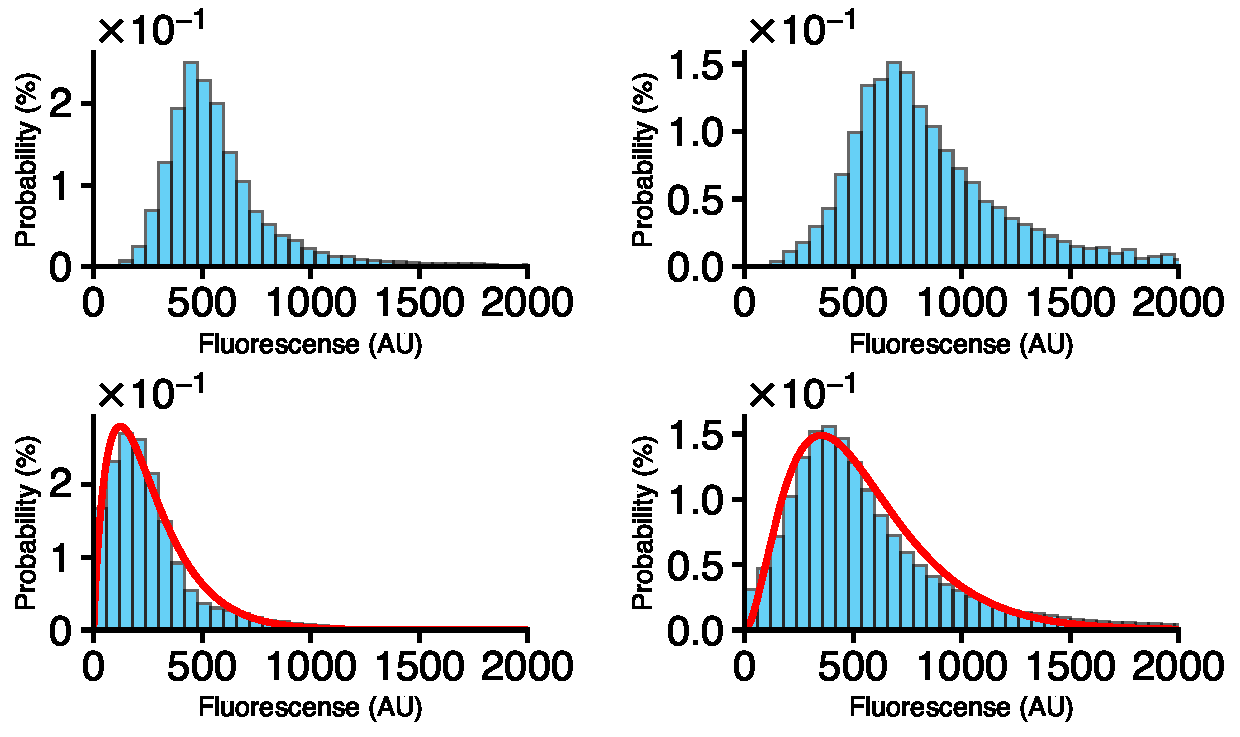
\includegraphics[width=0.67\linewidth]{assets/addendumFig2.pdf}
    \caption{Histograms of the measured fluorescence signals (top row) and their deconvolution results (bottom row) for \texttt{RAJ11\_100\_m26} (left) and \texttt{RAJ11\_100\_m32} (right). Bars depict the empirical probability distributions of the fluorescence intensities, while the red curves in the bottom panels represent fitted gamma distributions with the estimated shape and scale parameters.}\label{fig:figadd.2}
\end{figure}

%The fitted gamma distribution for wild-type had a moderate coefficient of variation (CV) with $\mathrm{CV}^2 \approx 0.63$ and skewness $\approx3.27$, indicating fluctuations somewhat lower than a Poisson process (which has $\mathrm{CV}^2=1$) despite bursty production. This suggests that frequent bursts (due to efficient sRNA binding) effectively even out protein production over time, reducing relative noise (analogous to noise buffering by microRNA regulation). In contrast, a mutant sRNA with weaker mRNA binding (RAJ11 A4T G5T) showed a more variable expression profile. Its protein distribution fit yielded $k\approx1.89$ (closer to exponential), and a nearly Poissonian noise level ($\mathrm{CV}^2\approx0.99$). The mutant's distribution maintained a similar mean fluorescence but with noticeably broader spread, consistent with more sporadic, less efficient bursting. An intermediate mutant (single base change, RAJ11 A4T) showed intermediate behavior (gamma $k\approx2.90$, $\mathrm{CV}^2\approx0.74$).

Key findings are that all sRNA-regulated cases produce right-skewed, bursty protein distributions, and weaker sRNA--mRNA interactions lead to higher noise (greater cell-to-cell variability) for a comparable mean output (\textbf{Fig. \ref{fig:figadd.1}}, \textbf{Fig. \ref{fig:figadd.2}}). These results quantitatively demonstrate post-transcriptional bursting in a real genetic system, in agreement with theoretical expectations \cite{Rodrigo2018}. Moreover, by fitting the distributions, we confirm that gamma-like forms appropriately describe the protein count variability, as seen previously in bursty gene expression systems. The wild-type sRNA effectively reduces relative noise and skewness compared to the weaker mutants, highlighting an intrinsic noise-control mechanism in the post-transcriptional bursting regime.

\section*{Discussion}
\subsection*{Mechanism of Post-Transcriptional Bursting}
Our preliminary findings suggest that that small RNAs can induce bursts of protein production by toggling translation on and off. In the RAJ11 system, the sRNA binding to the 5'UTR acts as a molecular switch: when bound, it exposes the Shine-Dalgarno sequence and triggers a period of active translation (the ``on'' state). Each binding event can generate a burst of protein until the complex dissociates or the mRNA is deactivated, at which point translation returns to ``off''. This mechanism is analogous to transcriptional bursting (where promoter states drive bursts of mRNA production) but occurs at the post-transcriptional level, downstream of mRNA synthesis. The derived burst frequency ($\sim k_{\text{on}}\langle s \rangle$) and burst size ($\sim k_p/k_{\text{off}}$) provide a useful intuitive picture: a higher sRNA concentration or binding rate increases how often bursts occur, while a slower unbinding (or inactivation) rate prolongs each translational burst, yielding more protein per burst.

Our incomplete analytical treatment (using Langevin equations and a telegraph process) is yet to reproduce these burst characteristics, consistent with previous stochastic models of gene expression bursts. Importantly, the post-transcriptional bursts we observe are a direct consequence of molecule-to-molecule variability at the RNA level (sRNA--mRNA interactions), rather than promoter state changes, which is consistent with the concept introduced by \cite{Rodrigo2018}: bursts of protein synthesis can arise ``beyond'' transcription, through dynamic RNA-level regulation.

In essence, an mRNA that is otherwise translationally silent can, upon sRNA binding, stochastically produce a flurry of protein, thereby increasing cell-to-cell heterogeneity in protein levels. Such bursts were evident in our experiments as heavy-tailed protein distributions. The right-skewed gamma distributions fitted to our data (with shape parameters $<$4) are indicative of infrequent large bursts and corroborate the idea that translational activation is episodic. These distributional signatures mirror those of classical transcriptional bursting -- for example, the negative binomial distributions reported for noisy gene expression in bacteria -- highlighting a unifying principle: bursting is a fundamental outcome of on/off dynamic regulation, whether at the promoter or post-transcriptional level.

\subsection*{Tuning of Expression Noise by sRNA--mRNA Interactions}
By comparing wild-type and mutant sRNAs, it is hinted that the kinetic parameters of sRNA binding (and unbinding) directly influence the magnitude of noise in protein expression. All variants produced similar mean protein levels in our conditions (owing to compensatory adjustments in burst frequency/duration), yet their noise profiles differed markedly. The wild-type sRNA, which has a strong binding affinity (large negative $\Delta G$ of binding), yielded a protein count distribution with lower normalized variance (CV) and moderate skewness. In contrast, the weakened-binding mutant (with seed mismatches) exhibited nearly Poisson-level noise and higher relative variance, even though the average protein output remained comparable. This trend suggests that strong sRNA binding ``smooths out'' protein production, making translation more constitutive at the single-cell level. %When binding is strong $k_\text{on}$ is high, bursts occur so frequently that they effectively overlap or the mRNA spends most of its time in the active state, leading to more steady protein accumulation (lower fractional noise).

%Conversely, when binding is weak (low $k_\text{on}$, high $k_\text{off}$), an mRNA infrequently enters the active state and for short durations, resulting in production that is bunched into rarer, brief bursts -- yielding higher cell-to-cell variability.

These observations resonate with studies of microRNA-based regulation in eukaryotes, where introducing an RNA-mediated repression can either buffer or amplify noise depending on kinetic regime \cite{Schmiedel2015}. In our bacterial case, the sRNA serves as an activator of translation, but the effect on noise is analogous: robust regulation (fast binding) buffers noise, whereas weaker regulation approaches the unregulated scenario of random translation initiation with full noise.

Notably, \cite{ArbelGoren2016} observed in an \textit{E. coli} sRNA network that noise is strongly influenced by sRNA-mediated mRNA decay and complex formation rates, which is consistent with our findings that altering sRNA--mRNA interaction strength modulates noise. Thus, our results bridge genotype (RNA sequence mutations) to phenotype (noise in protein levels): small changes in the seed region free energy (on the order of a few kcal/mol) can move the system from a relatively ``buffered'' expression regime to a highly stochastic one, without significantly changing mean expression. This tunability is of great interest for synthetic biology, as it offers a knob to adjust phenotypic variability independently of mean output \cite{Levine2007, Mutalik2012}.

Moreover, the ability to tune noise via RNA regulators supports the idea that cells could evolve or select for different noise levels by mutations in non-coding regions -- adding an evolutionary dimension to the role of post-transcriptional regulation.

\subsection*{Comparison to Transcriptional Bursting and Biological Implications}
It is insightful to compare the bursting we observe post-transcriptionally with the well-characterized phenomenon of transcriptional bursting. Transcriptional bursts (arising from promoters switching between inactive and active states) also produce heavy-tailed mRNA distributions and super-Poissonian noise \cite{Ozbudak2002}. In our post-transcriptional bursting, the ultimate protein distributions can be mathematically similar (e.g. both can often be described by negative binomial statistics), but the mechanistic origin is different: instead of promoter chromatin or transcription factor binding kinetics, it is the RNA-RNA interaction kinetics that set the burst parameters. One practical implication is in the timing and integration of cellular decisions. Transcriptional bursting is often implicated in fate determination events by providing occasional high transcript pulses. Post-transcriptional bursting could likewise generate heterogeneity in protein levels from uniformly transcribed mRNAs, thereby enabling phenotypic diversification without changes at the DNA level. This may be particularly relevant in stress responses or developmental contexts where small RNAs are known to play critical regulatory roles. Our results underscore that the RNA layer adds an additional opportunity for noise modulation in gene expression.

The distinctive feature of post-transcriptional bursts is that they can be rapidly tunable by introducing or modulating a regulatory RNA. In contrast, altering transcriptional burst kinetics often requires promoter mutations or changing transcription factor dynamics. From an evolutionary perspective, an organism might employ sRNA regulators to finetune expression noise on short evolutionary timescales (since RNA sequences can mutate to adjust binding affinity) while keeping the mean expression of a gene constant. This could be advantageous for bet-hedging strategies in fluctuating environments, or for coordinating multi-gene networks where only certain genes' expression noise needs adjustment. In summary, our study demonstrates that post-transcriptional bursting is a distinct but analogous phenomenon to transcriptional bursting, broadening the paradigm of how stochastic gene expression can arise. It highlights the often under-appreciated role of RNA interactions in generating phenotypic diversity, supporting the view that gene regulation at the RNA level is as significant as DNA-level regulation in shaping cellular heterogeneity.

Future investigations could explore the interplay of transcriptional and post-transcriptional bursts occurring together, and how cells orchestrate these layers of regulation to achieve desired expression dynamics \cite{Tanenbaum2014}. Our findings not only contribute to the fundamental understanding of gene expression noise but also provide design principles for constructing synthetic gene circuits with controllable noise via sRNA regulators.

\section*{Materials and Methods}
\subsection*{RAJ11 Construction Configuration}
The wild-type RAJ11 configuration deesigned on \cite{Rodrigo2015} comprises two core genetic elements: an sRNA module specifically designed to bind a complementary stretch of nucleotides (the ``toehold'') on the 5' UTR of the target mRNA, and a 5' UTR whose native secondary structure sequesters the ribosome-binding site (RBS). In the absence of the sRNA, this 5' UTR hairpin prevents ribosomes from accessing the RBS, resulting in minimal basal translation. The sRNA was computationally optimized in \cite{Rodrigo2015} to expose a highly accessible seed region that can quickly and stably hybridize to the 5' UTR. Once bound, the intramolecular hairpin in the mRNA is destabilized, making the RBS accessible for translation initiation. This design achieves tight cis-repression of the downstream GFP gene, followed by robust trans-activation only when the RAJ11 sRNA is present.

In addition to the wild-type RAJ11 configuration (referred to here as \texttt{RAJ11M}), we generated two key mutants, \texttt{RAJ11\_m26} and \texttt{RAJ11\_m32}, each introducing specific nucleotide substitutions that either modify the seed region of the sRNA or its complementary segment on the 5' UTR. For instance, \texttt{RAJ11\_m26} carries selected base changes in the sRNA seed to evaluate how disruptions in base-pair complementarity affect binding kinetics, whereas \texttt{RAJ11\_m32} alters nucleotides within the 5' UTR to test changes in RBS accessibility under partial or complete mismatch scenarios. By comparing the dynamic range of GFP expression across these constructs, we aimed to determine the extent to which each mutation weakens sRNA--mRNA pairing. This systematic set of mutants was instrumental for validating our thermodynamic predictions step by step, as it allowed us to link specific sequence changes to measurable shifts in translational activation.

Furthermore, we placed the \texttt{RAJ11M} configuration in both a high-copy-number plasmid (\texttt{RAJ11M}) and a low-copy-number plasmid (\texttt{RAJ11M\_P15}), and tested each under varying levels of anhydrotetracycline (ATC) induction, specifically 0 ng/mL (\texttt{RAJ11M}), 10 ng/mL (\texttt{RAJ11\_10}), and 100 ng/mL (\texttt{RAJ11\_100}). We then introduced the \texttt{RAJ11\_m26} and \texttt{RAJ11\_m32} mutants with 100 ng/mL of ATC (\texttt{RAJ11\_100\_m26} and \texttt{RAJ11\_100\_m32}). By comparing the resulting GFP outputs across these plasmid backgrounds and induction levels, we aimed to evaluate how increased sRNA transcription affects riboregulation in both wild-type and mutant variants.

\subsection*{Mathematical Model of sRNA-Mediated Gene Expression} We adopted the stochastic modeling framework described in \cite{Rodrigo2018} to describe a gene post-transcriptionally regulated by a small RNA. The system consists of an mRNA ($x$) and its protein product ($y$). Transcription of mRNA occurs with rate $k_m$, $c$ is the copy number of the gene, and translation of protein occurs only when the mRNA is in an active state (ribosome-binding site accessible) with rate $k_p$. The sRNA binding toggles this state. We formalized this using two coupled Langevin equations (Ito stochastic differential equations) for $x(t)$ and $y(t)$:

\begin{equation} \frac{dx}{dt} = c k_m - \gamma_m x + \sqrt{c k_m + \gamma_m x}\xi_m(t) \end{equation}

\begin{equation} \frac{dy}{dt} = k_p\zeta(t) - \gamma_p y + \sqrt{k_p,\zeta(t) + \gamma_p y}\xi_p(t) \end{equation}

where $\gamma_m$ and $\gamma_p$ are the degradation rates of mRNA and protein, respectively (so $1/\gamma_m$, $1/\gamma_p$ are their average lifetimes). The terms $\xi_m(t)$ and $\xi_p(t)$ represent independent Gaussian white noise processes (with $\langle \xi_i(t)\rangle=0$ and $\langle \xi_i(t)\xi_j(t')\rangle=\delta_{ij}\delta(t-t')$) accounting for intrinsic stochastic fluctuations.

The steady state solution for $\mathbb{E}[x(t)]$ is given by

\begin{align*}
    0 &= \mathbb{E}\left[c k_m - \gamma_m x + \sqrt{c k_m + \gamma_m x}\xi_m(t)\right]\\
    0 &= c k_m - \gamma_m \mathbb{E}[x]\\
    \mathbb{E}[x(t)] &= \frac{c k_m}{\gamma_m}
\end{align*}

We can only get this expression through 3 important assumptions:

\begin{enumerate} \item The noise term is zero on average (given by the white noise process). \item The amplitude of the stochastic process and the stochastic process are uncorrelated, hence the expectation of the product is the product of the expectations. \item We are using the mean-field approximation, i.e. the amplitude of the noise is finite, hence it disappears when multiplying by 0. \end{enumerate} Now that we have the expression for $\left\langle x\right\rangle$, we can substitute it back into the original equation by means of the mean-field approximation ($x = \left\langle x\right\rangle + \Delta x$):

\begin{align*}
    \frac{d\left(\mathbb{E}[x] + \Delta x(t)\right)}{dt} &= c k_m - \gamma_m\left(\mathbb{E}[x] + \Delta x(t)\right) + \sqrt{c k_m + \gamma_m\left(\mathbb{E}[x] + \Delta x(t)\right)}\xi_m(t)\\
    \frac{d\Delta x(t)}{dt} &= c k_m - \gamma_m\mathbb{E}[x] - \gamma_m\Delta x(t) + \sqrt{c k_m + \gamma_m\mathbb{E}[x]}\xi_m(t)\\
    \frac{d\Delta x(t)}{dt} &= -\gamma_m\Delta x(t) + \sqrt{2c k_m}\xi_m(t)
\end{align*}

To solve the above equation, we will use the Fourier transform of the equation. We'll denote the Fourier transform of $f$ as $\hat{f}$, equivalently as $\mathcal{F}\left\{f\right\}$. In this analysis, we assume that $\Delta x(t)$ is interpreted within the framework of tempered distributions, specifically belonging to the dual space $\mathcal{S}'(\mathbb{R})$ of the Schwartz space. This assumption guarantees that the Fourier transform is well-defined, even though white noise is not square-integrable in the classical sense.

\begin{align*}
    \mathcal{F}\left\{\frac{d\Delta x(t)}{dt}\right\} &= \mathcal{F}\left\{-\gamma_m\Delta x(t) + \sqrt{2ck_m}\xi_m(t)\right\}\\
    i\omega\hat{\Delta x}(\omega) - \Delta x_0&= -\gamma_m\hat{\Delta x}(\omega) + \sqrt{2ck_m}\hat{\xi}_m(\omega)\\
    \hat{\Delta x}(\omega) &= \left(\frac{\sqrt{2ck_m}}{i\omega + \gamma_m}\right)\hat{\xi}_m(\omega)
\end{align*}

This shows that the transfer function from noise to mRNA fluctuations is given by $G_x(i\omega) = \frac{\sqrt{2 c k_m}}{\gamma_m + i\omega}$. Note that we have proceeded with the assumption that the initial condition is zero ($\Delta x_0 = 0$). The next step of the derivation involves using the convolution theorem.

\begin{untheorem}[Convolution theorem]
    Let $f$ and $g$ be two functions with Fourier transforms $\hat{f}$ and $\hat{g}$, respectively. Then the convolution of $f$ and $g$, denoted as $f*g$ is given by:
    \begin{equation*}
        f(t)*g(t) = \mathcal{F}^{-1}\left\{\hat{f}(\omega)\hat{g}(\omega)\right\}
    \end{equation*}
\end{untheorem}

In simpler terms, the Fourier transform of the convolution of two functions equals the product of the Fourier transforms of each of the functions. In our particular case, we have 

\begin{equation*}
    \hat{\Delta x(\omega)} = \hat{g}(\omega)\hat{\xi}_m(\omega)
\end{equation*}

where $\hat{g}(\omega) = \left(\frac{\sqrt{2ck_m}}{i\omega + \gamma_m}\right)$. Therefore,

\begin{equation*}
    \Delta x(t) = \int_0^t\xi_m(\tau)g(t-\tau)d\tau
\end{equation*}

It is then necessary to compute the inverse Fourier transform of $\hat{g}(\omega)$. Our primary objectives are to verify the convergence of the integral obtained via the inverse Fourier transform and to explicitly address the behavior for $t<0$. In this context, we note that for $t<0$ the solution is defined to be zero, corresponding to the general form $H(t)e^{-\alpha t}$, where $H(t)$ is the Heaviside step function. Since the convolution integral is evaluated over the interval $(0,t)$, the case for $t<0$ is naturally excluded. The inverse Fourier transform of $\hat{g}(\omega)$ is given by:

\begin{align*}
g(t) &= \mathcal{F}^{-1}\left\{\hat{g}(\omega)\right\}\\
&= \left(\sqrt{2ck_m}\right)\mathcal{F}^{-1}\left\{\frac{1}{i\omega+\gamma_m}\right\}\\ 
&= \left(\sqrt{2ck_m}\right)\frac{1}{2\pi}\int_{-\infty}^{+\infty}\frac{1}{i\omega+\gamma_m}e^{i\omega t}d\omega
\end{align*}

Let's define $g(z) = \frac{1}{iz+\gamma_m}$, with $z\in\mathbb{C}$. We will introduce the following theorems:

\begin{untheorem}
    Suppose $f(z)$ is a function of $z\in\mathbb{C}$ and $f(z)$ is defined in the upper-half plane. If there is an $a>1$ and $M>0$ such that

    $$
    \left|f(z)\right| < \frac{M}{\left|z\right|^a}
    $$
  
    for a large $\left|z\right|$, then 
  
    $$
    \lim_{R\to\infty}\int_{C_R}f(z)dz = 0
    $$
  
    Where $C_R$ is the path (in this case an arch) that goes from $R$ in the real axis and goes back to $-R$ through the upper-half plane. This theorem is for functions that decay faster than $\frac{1}{z}$.
\end{untheorem}

\begin{untheorem}\label{theorem:complex_square}
    Suppose $f(z)$ is a function of $z\in\mathbb{C}$ and $f(z)$ is defined in the upper-half plane. If there is $M>0$ such that

    $$
    \left|f(z)\right| < \frac{M}{\left|z\right|}
    $$
  
    for a large $\left|z\right|$, then 
  
    $$
    \lim_{x_1\to\infty,x_2\to\infty}\int_{C_1+C_2+C_3}f(z)e^{iaz}dz = 0
    $$
  
    Where $C_1+C_2+C_3$ is a rectangular path that goes from point $x_1$ in the real axis up to the upper-half plane until height $(x_1+x_2)i$, then goes to the left until $-x_2$ and goes down to the real axis. This theorem is for functions that decay like $\frac{1}{z}$.
\end{untheorem}

For our particular case, we'll use the previous theorem (as we can see that $g(z)$ decays like $\frac{1}{z}$). So, we need to find a value of $M>0$ so that the bound holds:

\begin{align*}
\left|g(z)\right| &= \left|\frac{1}{iz+\gamma_m}\right|\\
&= \frac{1}{\left|iz+\gamma_m\right|}\\
&= \frac{1}{\sqrt{(\text{Re}(z))^2 + (\gamma_m - \text{Im}(z))^2}}\\
&= \frac{1}{\sqrt{\gamma_m^2 - 2\gamma_m\text{Im}(z) + \text{Re}^2(z) +\text{Im}^2(z)}}\\
&= \frac{1}{\sqrt{\gamma_m^2 - 2\gamma_m\text{Im}(z) + \left|z\right|^2}}\\
\end{align*}

for a large $\left|z\right|$, we can see that $\left|g(z)\right| \approx \frac{1}{\left|z\right|}$, so we can use the theorem as any $M>1$ is sufficient to make the bound hold:

\begin{align*}
\left|g(z)\right| &= \frac{1}{\sqrt{\gamma_m^2 - 2\gamma_m\text{Im}(z) + \left|z\right|^2}}\\
&\approx \frac{1}{\left|z\right|} < \frac{M}{\left|z\right|}\\
\end{align*}

With this condition met, we can use the standard contour $C_1+C_2+C_3 + C_4$ which forms a rectangle that goes from point $x_1$ in the real axis up to the upper-half plane until height $(x_1+x_2)i$, then goes to the left until $-x_2$, then goes down to the real axis and finally goes back to our starting point. Note then that if we take the limits $x_1\to\infty$ and $x_2\to\infty$ on contour $C_4$, we have our original integral (the one from the inverse Fourier transform):

$$
\lim_{x_1\to\infty, x_2\to\infty}\int_{C_4}g(z)e^{iaz}dz = \lim_{x_1\to\infty, x_2\to\infty}\int_{-x_2}^{x^1}\frac{e^{iz t}}{iz+\gamma_m}dz
$$

Furthermore, given the bound $M > 1$ we know that

$$
\lim_{x_1\to\infty, x_2\to\infty}\int_{C_1+C_2+C_3}g(z)e^{iaz}dz = 0
$$

Therefore, the entire contour integral over $C_1 + C_2 + C_3 + C_4$:

\begin{align*}
\lim_{x_1\to\infty, x_2\to\infty}\int_{C_1+C_2+C_3+C_4}g(z)e^{iaz}dz &= 0 + \lim_{x_1\to\infty, x_2\to\infty}\int_{C_4}\frac{e^{izt}}{iz+\gamma_m}dz
\end{align*}

So, the inverse Fourier transform is given by the contour integral over $C_1 + C_2 + C_3 + C_4$. We can then use the residue theorem to compute the integral.

\begin{untheorem}[Cauchy's Residue Theorem]
    Let $f(z)$ be a function that is analytic in a region $D$ except for a finite number of isolated singularities. For any simple closed curve $C$ that is positively oriented and lies in $D$:
    $$
    \oint_C f(z)dz = 2\pi i\sum_{k=1}^{n} \text{Res}(f,z_k)
    $$
    where $z_k$ are the singularities of $f(z)$ in $D$ and $\text{Res}(f,z_k)$ denotes the residue of $f$ at $z_k$.
\end{untheorem}

The residue of a function $f(z)$ at a point $z_0$ is given by:

$$
\text{Res}(f,z_0) = \lim_{z\to z_0} (z-z_0)f(z)
$$

In our case, we have a simple pole at $z = \gamma_m i$, as the denominator of $g(z)$ is zero at $z = \gamma_m i$. Since $\gamma_m > 0$, we have that the pole is in the upper-half plane. In addition, the pole is a simple pole, we can compute the residue through the definition:

\begin{align*}
\text{Res}(g,\gamma_m i) &= \lim_{z\to \gamma_m i} (z-\gamma_m i)\left(\frac{e^{izt}}{iz+\gamma_m}\right)\\
&= e^{-\gamma_mt}\lim_{z\to \gamma_m i} \left(\frac{z-\gamma_m i}{iz+\gamma_m}\right)\\
&= \frac{e^{-\gamma_mt}}{i}\lim_{z\to \gamma_m i} \left(\frac{iz +\gamma_m}{iz+\gamma_m}\right) = \frac{e^{-\gamma_mt}}{i} = -ie^{-\gamma_mt}\\
\end{align*}

Now we can use Cauchy's Residue Theorem to compute the integral:

\begin{align*}
\int_{C_4}\frac{e^{iz t}}{iz+\gamma_m}dz &= 2\pi i\text{Res}(g,\gamma_m i)\\
&= 2\pi i\left(-ie^{-\gamma_mt}\right)\\
&= 2\pi e^{-\gamma_mt}
\end{align*}

Returning to the inverse Fourier transform, we have:

\begin{align*}
g(t) &= \left(\sqrt{2ck_m}\right)\left(\frac{1}{2\pi}\int_{-\infty}^{\infty}\frac{e^{i\omega t}}{i\omega+\gamma_m}d\omega\right)\\
&= \sqrt{2ck_m}e^{-\gamma_mt}
\end{align*}


Therefore, the general solution for $\Delta x(t)$ is given by:

\begin{align*}
\Delta x(t) &= \int_0^t \xi_m(\tau)g(t-\tau)d\tau\\
&= \sqrt{2ck_m}\int_0^t \xi_m(\tau)e^{-\gamma_m(t-\tau)}d\tau
\end{align*}

Besides the above, we can also compute the spectral density of $\Delta x(t)$, which we'll denote as $S_{\Delta x}$. The spectral density is defined as the squared absolute value of the Fourier transform of the process. So for our process, we have that

\begin{align*}
S_{\Delta x} &= \left|\mathcal{F}\left\{\Delta x\right\}\right| = \left|\hat{\Delta x}\right|^2\\
&= \left|\sqrt{2ck_m}\left(\frac{1}{i\omega+\gamma_m}\right)\hat{\xi}_m(\omega)\right|^2\\
&= \left(\frac{2ck_m}{\omega^2+\gamma_m^2}\right)\left|\hat{\xi}_m(\omega)\right|^2\\
\end{align*}

Do note that one needs to be extra careful when using these definitions, because the Fourier transform of white noise process is defined only as a kind of limit of smooth processes. Fortunately, as long as we only work with linear systems this definition indeed works. And it provides a useful tool for determining covariance functions of stochastic differential equations.

A great property is that, since the Fourier transform of white noise is a constant (imagine a white noise signal in the time domain; it appears as a random fluctuation where the amplitude changes rapidly and unpredictably. When the Fourier transform of this signal is taken to analyze its frequency components, it can be seen that there is no preference for any specific frequency; all frequencies are equally likely to contribute to the noise), the spectral density of the process is also a constant.

Therefore

\begin{align*}
S_{\Delta x} &= \left(\frac{2ck_m}{\omega^2+\gamma_m^2}\right)\left|\hat{\xi}_m(\omega)\right|^2\\
&= \frac{2ck_m}{\omega^2+\gamma_m^2}\\
\end{align*}


Next we need to introduce the Wiener-Khinchin theorem.

\begin{untheorem}[Wiener-Khinchin]
    For a wide-sense stationary random process, the power spectral density $S_x(\omega)$ and the autocorrelation function $C_x(t)$ form a Fourier transform pair:
    $$
    S_x(\omega) = \mathcal{F}\{C_x(t)\} \quad \text{and} \quad C_x(t) = \mathcal{F}^{-1}\{S_x(\omega)\}
    $$
    where $\mathcal{F}$ denotes the Fourier transform and $\mathcal{F}^{-1}$ its inverse.
\end{untheorem}

Let's denote the autocorrelation function of $\Delta x(t)$ as $C_{\Delta x}$, so by means of the Wiener-Khinchin theorem, we have that

\begin{align*}
C_{\Delta x} &= \mathcal{F}^{-1}\left\{S_{\Delta x}\right\}\\
&= \mathcal{F}^{-1}\left\{\frac{2ck_m}{\omega^2+\gamma_m^2}\right\}\\
&= \frac{2ck_m}{2\gamma_m}\mathcal{F}^{-1}\left\{\frac{2\gamma_m}{\omega^2+\gamma_m^2}\right\}\\
&= \frac{ck_m}{\gamma_m}e^{-\gamma\left\lvert \Delta t\right\rvert}
\end{align*}

Note that the inverse Fourier transform here was computed using the property of the Fourier transform being a linear operator, and using the known result that $\mathcal{F}^{-1}\left\{\frac{2\alpha}{\alpha^2 + \omega^2}\right\} = e^{\alpha\left\lvert t\right\rvert}$

With these definitions, it is left to compute the statistical properties of the protein $y(t)$, which is left unsolved as this work is yet to be published.

% The key state variable $\zeta(t)$ is a two-state (0/1) telegraph process representing whether an mRNA is translationally active at time $t$. Specifically, $\zeta=0$ corresponds to the mRNA's ribosome-binding site being occluded (translation ``off''), and $\zeta=1$ corresponds to the mRNA being bound by sRNA in such a way that the ribosome-binding site is exposed (translation ``on''). The switching of $\zeta$ is governed by the sRNA--mRNA interaction kinetics.: we denote $k_{\text{on}}$ as the rate at which an inactive mRNA becomes active (sRNA binding or action) and $k_{\text{off}}$ as the rate at which an active mRNA returns to inactive (sRNA unbinding or complex inactivation). In steady state, $\zeta(t)$ has an average value equal to the fraction of time an mRNA is in the on state. We define $p_{\text{on}} = \frac{k_{\text{on}}\langle s\rangle}{k_{\text{on}}\langle s\rangle + k_{\text{off}}}$ as the equilibrium probability an mRNA is active (here $\langle s\rangle$ is the average free sRNA concentration). The autocorrelation of the telegraph process decays with a characteristic time $\tau \approx (k_{\text{on}}\langle s\rangle + k_{\text{off}})^{-1}$, and for an ideal telegraph one has $\langle \zeta(t)\zeta(0)\rangle - \langle \zeta \rangle^2 \propto e^{-t/\tau}$. In our model, we set $\langle \zeta(t)\rangle = \langle x \rangle p_{\text{on}}$ to reflect that the number of active mRNAs is bounded by total mRNAs.

% We note that this formulation effectively assumes the sRNA is present and dynamically binding; in the absence of sRNA, $p_{\text{on}}\to0$ and translation events are negligible. To analyze the model, we first solved for the steady-state mean mRNA. Setting $d\langle x\rangle/dt=0$ in the mRNA equation and using $\langle \xi_m(t)\rangle=0$, we obtain $0 = c k_m - \gamma_m \langle x\rangle$, hence $\langle x\rangle = c k_m/\gamma_m$. This result relies on the mean-field approximation that $\langle \sqrt{\gamma_m x},\xi_m\rangle = 0$ (justified by the noise being zero-mean and uncorrelated with amplitude to first order). We then performed a fluctuation analysis by writing $x(t) = \langle x\rangle + \Delta x(t)$ and linearizing. This yields an Ornstein--Uhlenbeck type equation for the mRNA fluctuations:

% \begin{equation}
%     d(\Delta x)/dt \approx -\gamma_m \Delta x + \sqrt{2c k_m},\xi_m(t)    
% \end{equation}

% after substituting $\langle x\rangle$ into the noise term. The solution of this linear stochastic differential equation was obtained via Fourier transform methods. In the frequency domain, the transfer function from noise $\xi_m$ to mRNA output $\Delta x$ is $G_x(i\omega) = \frac{\sqrt{2 c k_m}}{\gamma_m + i\omega}$. From this, we computed the mRNA power spectral density and autocorrelation, confirming that mRNA fluctuations follow an exponential relaxation with correlation time $1/\gamma_m$ (consistent with a simple birth--death process). These analytical results (notably, that the Fano factor of mRNA is 1 at steady state, as expected for a Poissonian transcript process) provided a baseline for understanding how translational bursting influences the protein statistics. For the protein $y(t)$, the production term is modulated by $\zeta(t)$. Rather than deriving an explicit analytical solution for $y(t)$ (which leads to a system of integro-differential equations due to the two-state switching), we utilized stochastic simulation to capture the protein burst statistics. We implemented Gillespie's exact stochastic simulation algorithm (SSA) \cite{Gillespie2007} to generate trajectories of the coupled $(x,\zeta,y)$ system. In the SSA, transcription, translation (when $\zeta=1$), switching on, and switching off are treated as reaction channels with propensities $c k_m$, $k_p x$ (active only if $\zeta=1$), $k_{\text{on}} s x$ (sRNA binds an available mRNA; we update $s$ accordingly if tracking sRNA pool), and $k_{\text{off}} x_{\text{active}}$ (active mRNA switches off) respectively. Each simulation step advances the system by sampling the next reaction and time increment from exponential waiting-time distributions.

% Parameter values were chosen in line with prior experimental and modeling studies of bacterial gene expression. We used $c=1$ (single-copy gene). The transcription rate $k_m$ and decay rate $\gamma_m$ were set such that $\langle x \rangle$ is on the order of 1--10 mRNAs per cell (a few transcripts per cell, typical for low-expression genes). The translation rate $k_p$ and protein decay (dilution) rate $\gamma_p$ were set to yield mean protein levels in the range of tens to a few hundred per cell (matching the scale of our fluorescence measurements). For instance, in dimensionless units, we often took $\gamma_m=1$,min$^{-1}$, $k_m=1$,min$^{-1}$ (so $\langle x\rangle=1$ mRNA), $k_p=20$,min$^{-1}$, and $\gamma_p=0.05$,min$^{-1}$ (protein half-life on the order of hours), although for the RAJ11 constructs the effective protein degradation includes dilution in dividing \textit{E. coli}, so $\gamma_p \sim 0.02$--0.03,min$^{-1}$. The on/off switching rates were inferred from thermodynamic calculations (see below) but tested in simulations over a range consistent with those free energies. We simulated long enough to collect stable protein distributions (typically $>10^4$ minutes, discarding transients).

% \subsection*{Thermodynamic Analysis of sRNA--mRNA Interactions}

% To parameterize $k_{\text{on}}$ and $k_{\text{off}}$ for the RAJ11 sRNA--mRNA pair and its mutants, we performed RNA secondary structure and free energy calculations. We used NUPACK (v4) to compute the minimum free energy (MFE) structures for: (i) the 5'UTR of the mRNA alone (cis-RAJ11), (ii) the sRNA alone (trans-RAJ11), and (iii) the sRNA--mRNA duplex (co-folded complex). The wild-type sequences and two mutant sRNA sequences (with seed region mutations A4U and G5U, individually and combined) were analyzed. The MFE of the mRNA alone ($\Delta G_m$) was found to be -14.4 kcal/mol, corresponding to a hairpin that sequesters the ribosome binding site (SD sequence). The sRNA alone has a stable structure ($\Delta G_s \approx -37.1$ kcal/mol).

% For the sRNA--mRNA complex, we obtained an overall free energy $\Delta G$ (duplex formation) and an activation free energy $\Delta G^\ddagger$ associated with initiating the interaction \cite{Rodrigo2015}. For wild-type RAJ11, the duplex MFE was $\Delta G \approx -14.5$ kcal/mol, roughly equal (in magnitude) to the mRNA hairpin energy, implying the complex formation just compensates the cost of opening the mRNA hairpin. The reported $\Delta G^\ddagger$ for this interaction was about -10.3 kcal/mol. For the single-mutant sRNA (A4U), the duplex MFE was weaker ($\Delta G \approx -10.1$ kcal/mol) and the effective $\Delta G^\ddagger \approx -5.9$ kcal/mol. The double-mutant (A4U G5U) showed a substantially reduced binding stability: $\Delta G \approx -6.5$ kcal/mol and $\Delta G^\ddagger \approx -3.7$ kcal/mol. These thermodynamic parameters indicate that the mutant sRNAs have lower affinity for the target mRNA and likely slower binding kinetics. We leveraged these values to estimate the kinetic rates using an Arrhenius/Kramers approach \cite{Hanggi1990}. In this scheme, we set:

% \begin{equation}
%     k_{\text{on}} = A \exp(-\Delta G^\ddagger/RT) 
% \end{equation}

% \begin{equation}
%     k_{\text{off}} = A \exp(-(\Delta G^\ddagger - \Delta G)/RT)
% \end{equation}

% where $A$ is a frequency factor (related to diffusion-limited collision frequency, set on the order of $10^6$--$10^7$ M$^{-1}$s$^{-1}$ for RNA interactions in the cell) and $RT$ is the thermal energy (we assume $T=310$ K, so $RT\approx0.616$ kcal/mol). This nonequilibrium two-state model ensures that the ratio $k_{\text{on}}/k_{\text{off}} = \exp(-\Delta G/RT)$, matching the equilibrium binding constant from the free energy of duplex formation. We used the above relations to compute baseline $k_{\text{on}}$ and $k_{\text{off}}$ for simulations: for wild-type, $\Delta G^\ddagger - \Delta G \approx 4.2$ kcal/mol, so if we assume a modest $A$ (yielding $k_{\text{on}}$ on the order of $0.1$ min$^{-1}$), we get $k_{\text{off}}$ roughly one order of magnitude smaller (favoring the on-state). For the weakest mutant, $\Delta G^\ddagger - \Delta G \approx 3.7 - (-6.5) = 10.2$ kcal/mol (if interpreted directly, but note $\Delta G^\ddagger$ was given negative; in practice the barrier for binding is much higher relative to the net gain), leading to a much larger $k_{\text{off}}/k_{\text{on}}$ ratio. In qualitative terms, wild-type is expected to spend most time in the active state (high $p_{\text{on}}$), whereas the mutant might have $p_{\text{on}} \ll 1$ under similar sRNA concentrations. These rates were fed into the SSA simulations and also used in theoretical calculations of expected burst statistics.

\subsection*{Data Collection and Analysis}
For experimental validation, \textit{E. coli} cells carrying the RAJ11 construct were analyzed by flow cytometry. The construct consisted of a reporter gene with the cis-RAJ11 5'UTR and a constitutive promoter, and sRNA (trans-RAJ11) expressed from a regulated promoter. We collected single-cell fluorescence distributions for: (1) no sRNA (sRNA promoter off), (2) wild-type sRNA (induced to a certain level, labeled ``100'' which corresponds to a saturating inducer concentration), and (3) two sRNA mutants (with the same induction level). Three biological replicate samples were measured for each condition. To isolate the true protein signal distribution, we performed a deconvolution to subtract autofluorescence. The autofluorescence (background fluorescence of cells with no reporter) was measured and its distribution $b(x)$ obtained as a histogram. The raw fluorescence distribution with the reporter (which includes both background and reporter signal) is denoted $a(x)$. We treated the relationship as a convolution $a(x) = (b * c)(x)$, where $c(x)$ is the sought distribution of true reporter signal.

We implemented the deconvolution in Python by constructing the convolution matrix $B$ for $b$ and solving the linear system $B,\hat{c} = a$ for $\hat{c}$ (discrete approximation of the convolution equation). Because this inverse problem is ill-posed and $B$ is non-square, we obtained a least-squares solution with Tikhonov regularization (ridge regression) to enforce smoothness and non-negativity. Specifically, we solved $(B^T B + \lambda I)\hat{c} = B^T a$ with regularization parameter $\lambda=1$ (chosen empirically to suppress high-frequency noise in $\hat{c}$ without over-smoothing). The solution $\hat{c}(x)$ was taken as the deconvolved probability density of cellular fluorescence due to the reporter. We validated the deconvolution by reconvolving $\hat{c}$ with $b$ to obtain $\hat{a}$ and comparing it to the measured $a$. The coefficient of determination $R^2$ between $a$ and $\hat{a}$ was above 0.95 in all cases, indicating a good fit. We also computed a $t$-statistic to confirm that $\hat{c}$ significantly improved the fit over a null model. 

The deconvolved distributions $\hat{c}(x)$ for each condition were then analyzed to extract quantitative descriptors of bursting. We fit each distribution with a gamma distribution, $P(x) = x^{k-1}e^{-x/\theta}/[\Gamma(k)\theta^k]$, using maximum likelihood (via SciPy's \texttt{fit} function). This provided the shape parameter $k$ and scale $\theta$ for each condition, along with estimates of uncertainty. The fits were visually excellent and yielded $R^2>0.95$ in each case. From the theoretical distribution and from the raw data, we calculated the mean, variance, noise (defined as variance divided by mean squared, $\mathrm{CV}^2$), and skewness for each condition. These higher moments characterize bursty distributions: a Poisson distribution has $\mathrm{CV}^2=1$ and skewness = 1 (if treated as counts); higher values indicate more burstiness/variability. We found skewness strictly higher than 1 for all cases, indicating that the distributions are indeed bursty. Nonetheless, further analysis of the data is needed to confirm the validity of the theoretical model.

% The wild-type sRNA condition showed the lowest noise and a higher effective burst size (since its gamma shape $k$ was highest), whereas the mutant with two seed mismatches showed nearly Poisson noise (indicating bursts are minimal, translation events largely independent). These metrics were consistent with the qualitative behavior observed in simulations. All analyses were conducted in Python 3.8 using numpy, pandas, and SciPy; plots were generated with matplotlib. Where appropriate, we cross-validated the simulation results with the analytical model (e.g., ensuring the mean expressions and trends in noise vs. binding strength matched predictions). We also compared our results with prior literature to ensure our definitions of noise and burst statistics were standard. The combination of theoretical modeling, simulation, and experimental distribution deconvolution allowed us to rigorously characterize post-transcriptional bursting in the RAJ11 system.
\vfill
\section*{Conclusions}
This work takes a glipse into the pivotal role of sRNA-induced post-transcriptional regulation in shaping gene expression variability, looking to complement the well-characterized phenomenon of transcriptional bursting. Drawing on our modeling framework, single-cell fluorescence data, and the systematic exploration of wild-type vs. mutant sRNA constructs, we seek to demonstrate that sRNA-mediated translational on/off switching can yield robust bursts of protein production and generate heavy-tailed protein distributions. We envision these results to add depth to our understanding of multiscale biological noise: while transcriptional events can encode bursts at the mRNA level, the additional sRNA layer provides another point at which stochastic fluctuations may be amplified, modulated, or buffered. 

These fluctuations, in turn, do contribute to a hierarchical cascade of noise propagation, where molecular-level stochasticity accumulates and integrates across multiple regulatory layers to ultimately shape macroscopic phenotypic variation. This multi-level aggregation of noise sources parallels other biological phenomena where microscopic randomness gives rise to emergent stochastic behaviors at larger scales -- from protein conformational dynamics to evolutionary trajectories. Indeed, just as the superposition of multiple noise sources in gene expression can lead to non-Poissonian statistics and complex temporal patterns, the integration of various molecular-level mutational processes across different genes can collectively drive anomalous diffusion-like behaviors in evolutionary dynamics. Understanding these connections between microscopic stochasticity and macroscopic phenomenology is crucial for developing accurate quantitative models of biological variation across scales, and is yet to be fully uncovered.

\vfill

\pagebreak

\bibliographystyle{assets/rodrigostyle}
\bibliography{references/addendumReferences}
